\begin{center}
\Huge
Tangenter
\end{center}
\section*{Mere om tangenter}
\stepcounter{section}
\begin{exa}
Vi betragter funktionen 
\begin{align*}
f(x) = x^3-3x^2+2x+1.
\end{align*}
Vi ønsker at finde ligningen for alle de tangenter til $f$, der har hældning $2$. Vi finder først den afledede til $f$:
\begin{align*}
f'(x) = 3x^2-6x+2.
\end{align*}
Vi skal løse ligningen $f'(x)=2$, da vi så vil finde $x$-værdien alle de steder, der har hældning lig 2.
\begin{align*}
3x^2-6x+2 = 2\  \Leftrightarrow \ 3x^2-6x=0 \Leftrightarrow x=0 \ \vee \ x = 2.
\end{align*}
Vi finder den tilhørende $y$-værdi til disse punkter:
\begin{align*}
f(x=0) &= 1,\\
f(x=2) &= 1.
\end{align*}
Vi ved derfor at tangenterne skal gå gennem henholdsvist punkterne $(0,1)$ og $(2,1)$. Vi kan derfor løse for $b$-værdien i tangentens ligning $y = 2x+b$.
\begin{align*}
y_1 = 2x+b_1 \ \Leftrightarrow\  1 = 2\cdot 0 + b_1 \Leftrightarrow\  b_1 = 1,\\
y_2 = 2x+b_2 \ \Leftrightarrow\  1 = 2\cdot 2 + b_2 \Leftrightarrow\  b_2 = -3.
\end{align*} 
Derfor har tangenterne til funktionen $f$ med hældning $2$ ligningerne 
\begin{align*}
y = 2x+1,\\
y = 2x -3.
\end{align*}
Dette kan ses på Fig. \ref{fig:dobbelttangent}.
\begin{figure}[H]
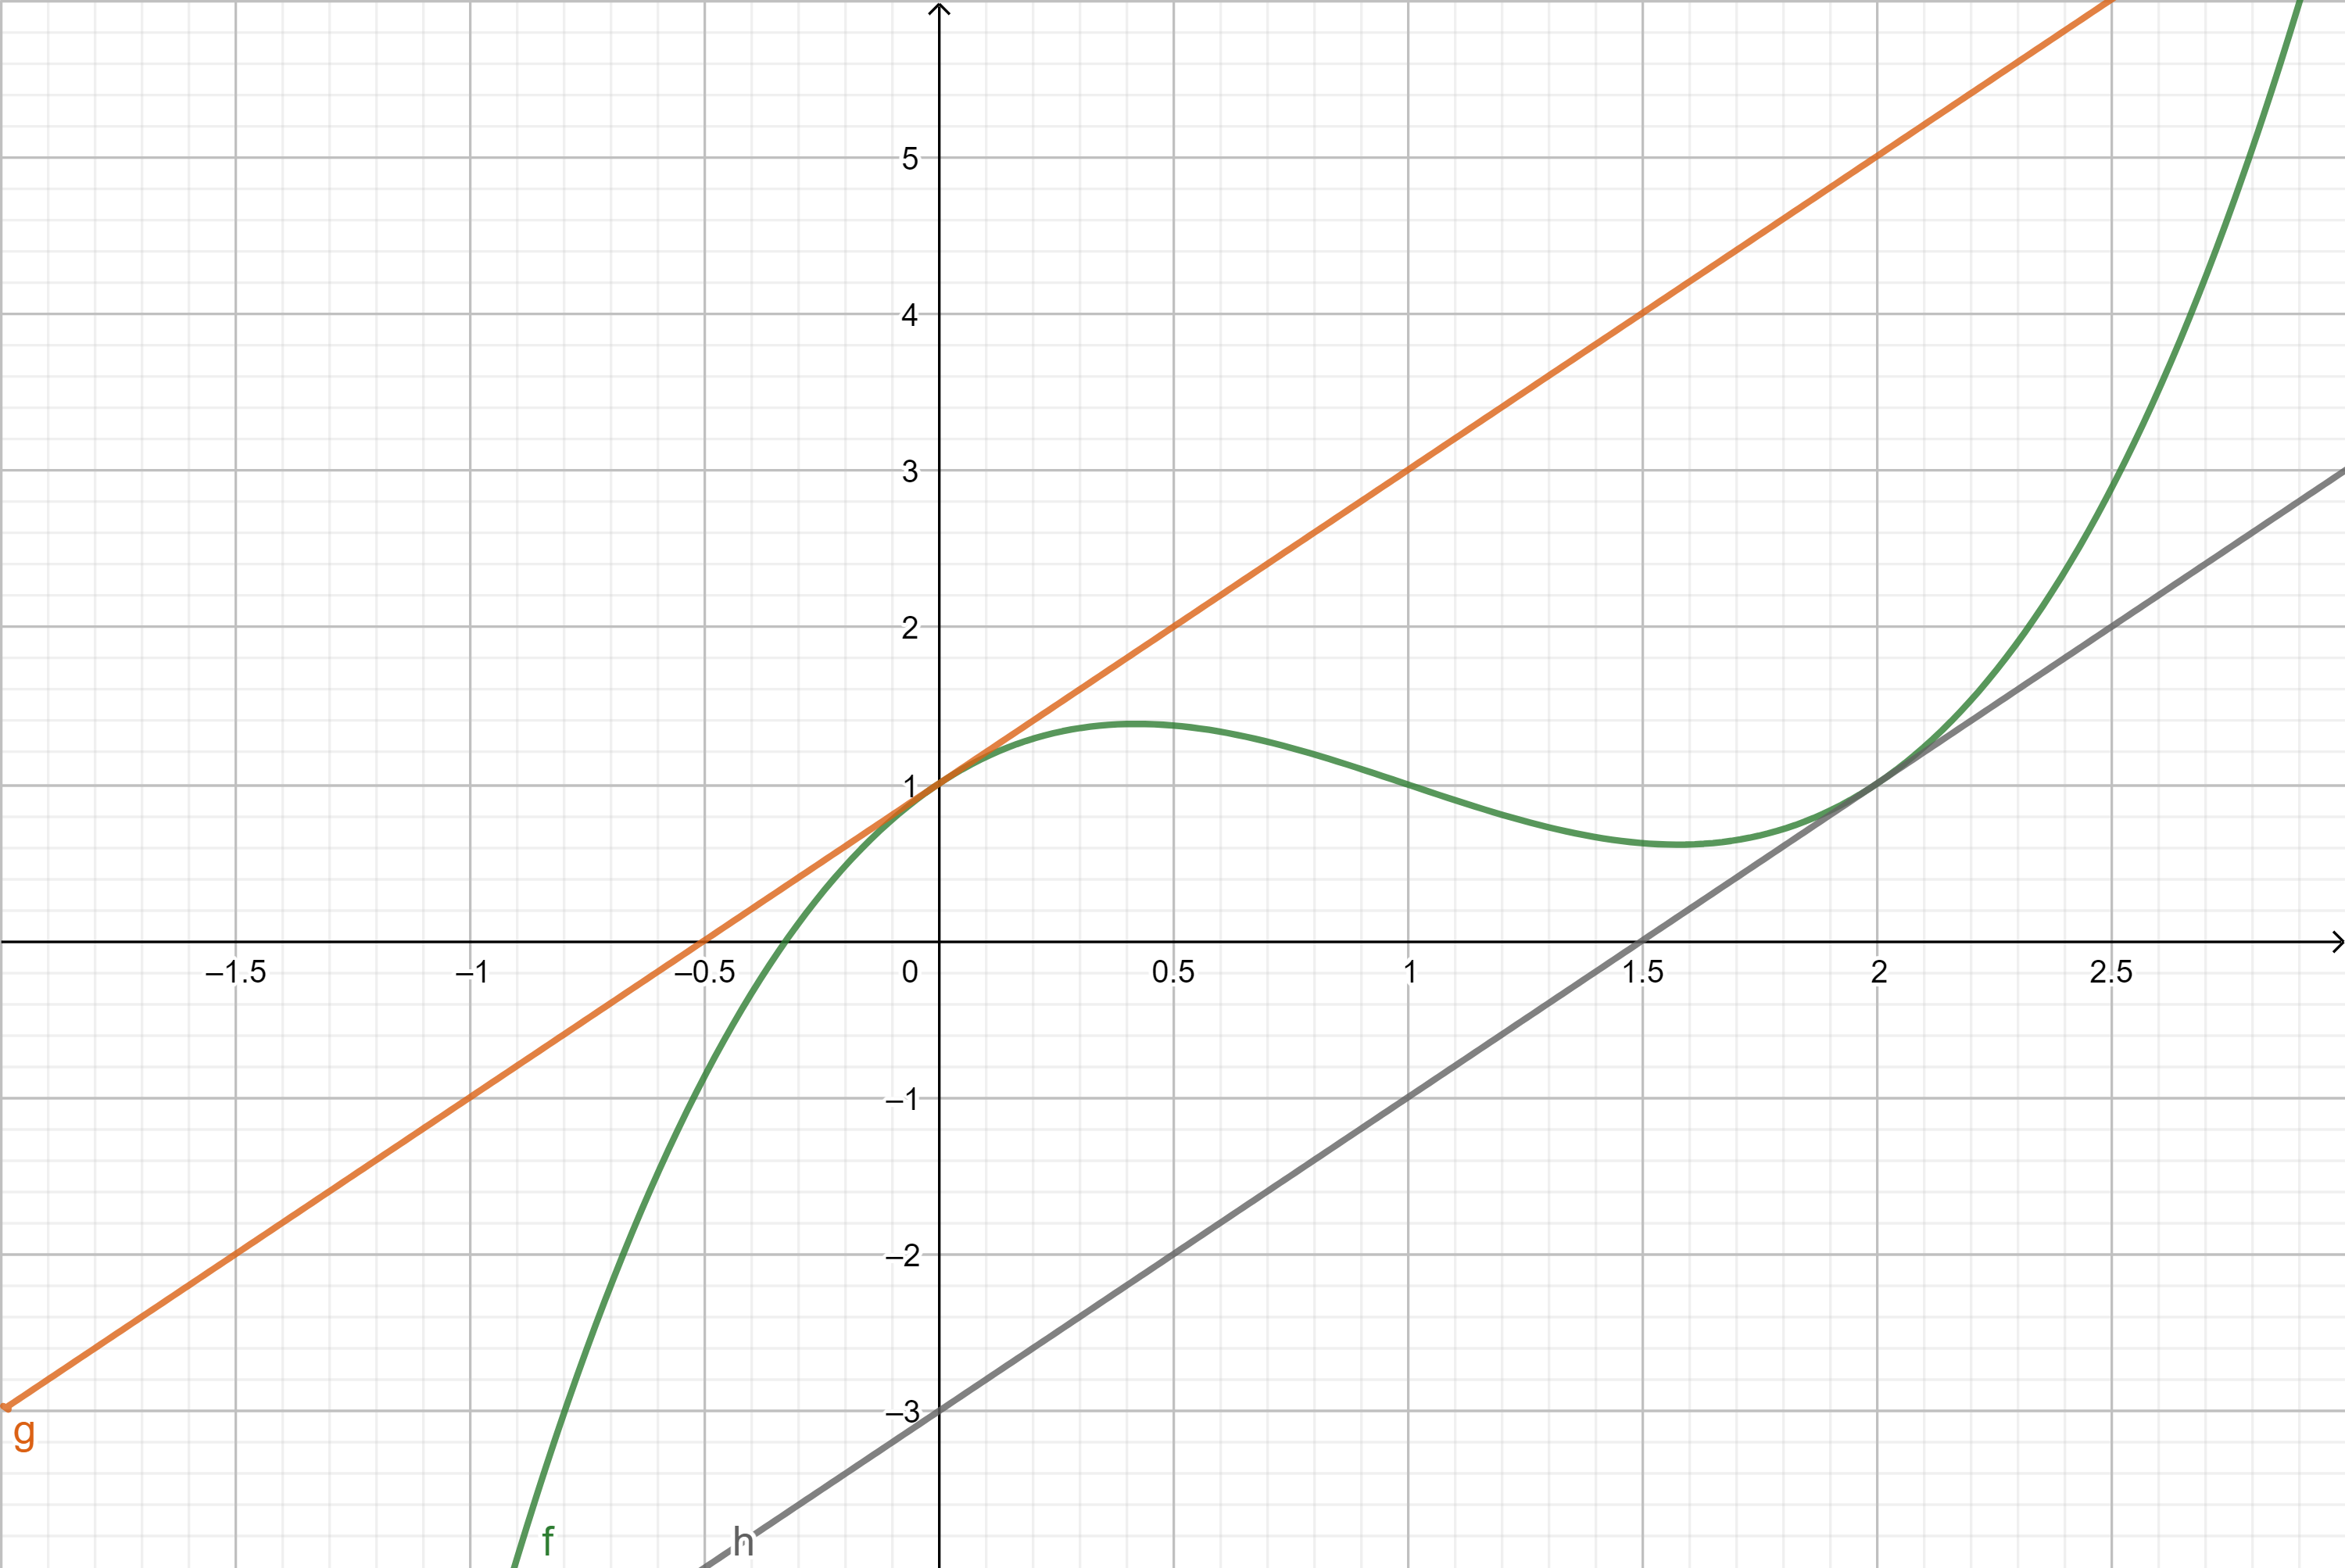
\includegraphics[width = 10cm]{Billeder/dobbelttangent.png}
\centering
\caption{Funktionen $f$ med de to tangenter, der har hældning $2$.}
\label{fig:dobbelttangent}
\end{figure}
\end{exa}

\section*{Differentialkvotient for $\frac{1}{x}$}
\stepcounter{section}
\begin{setn}
Funktionen $f(x) = \frac{1}{x}$ er differentiabel så længe $x\neq 0$, og differentialkvotienten er givet
\begin{align*}
f'(x) = -\frac{1}{x^2}.
\end{align*}
\end{setn}
\begin{proof}
Antag, at $x\neq 0$. Vi anvender definitionen af differentialkvotienten:
\begin{align*}
f'(x) = \lim_{h\to 0} \frac{f(x+h)-f(x)}{h}.
\end{align*}
I tilfældet at $f(x) = \frac{1}{x}$ får vi så
\begin{align*}
(\frac{1}{x})' &= \lim_{h\to 0} \frac{\frac{1}{x+h}-\frac{1}{x}}{h}\\
&= \lim_{h\to 0} \frac{\frac{x-(x+h)}{(x+h)x}}{h}\\
&= \lim_{h\to 0} \frac{-h}{x(x+h)h}\\
&= \lim_{h\to 0} \frac{-1}{x(x+h)}.
\end{align*}
Da $x\neq 0$ er $\frac{-1}{x(x+h)}$ kontinuert i $x$. Derfor får vi, at 
\begin{align*}
 \lim_{h\to 0} \frac{-1}{x(x+h)} = -\frac{1}{x^2}.
\end{align*}
\end{proof}
\begin{setn}
Funktionen $f(x) = x^3$ er differentiabel overalt og differentialkvotienten for $f$ er givet ved
\begin{align*}
f'(x) = (x^3)' = 3x^2
\end{align*}
\end{setn}
\begin{proof}
Vi anvender som før definitionen af differentialkvotienten for $f$:
\begin{align*}
(x^3)' &= \lim_{h\to 0}\frac{(x+h)^3-x^3}{h}\\
       &= \lim_{h\to 0}\frac{(x+h)(x^2+h^2+2xh)-x^3}{h}\\
       &= \lim_{h\to 0}\frac{x^3+xh^2+2x^2h+hx^2+h^3+2xh^2-x^3}{h}\\
       &= \lim_{h\to 0}\frac{xh^2+2x^2h+hx^2+h^3+2xh^2}{h}\\
       &= \lim_{h\to 0}xh+2x^2+x^2+h^2+2xh\\
       &= 2x^2+x^2 = 3x^2.
\end{align*}
\end{proof}

\section*{Opgave 1}
Find alle de steder, hvor følgende funktioner har den givne tangenthældning:
\begin{align*}
&1) \ f(x) = x^2,\  f'(x) = 0     &&2) \ f(x) = 3x^2 + 2x + 1,\  f'(x) = 2    \\
&3) \ f(x) = x^3-5x+10, \ f'(x) = 7    &&4) \ f(x) = 2x^3 -2x^2+10x+3, \ f'(x) = 1     \\
&5) \  f(x) = x^3-10x^2+10x+1,\ f'(x) = -5   &&6) \ f(x) = -x^2+13x+2, f'(x) = -4    
\end{align*}
\section*{Opgave 2}
\begin{enumerate}[label = \roman*)]
\item Find ligningen for tangenten til funktionen $f(x)=-2 x^3-10x^2+2x+1$ i punktet $(-4,f(-4))$. Har denne funktion andre tangenter, der er parallelle til denne tangent?
\item Find ligningen for tangenten til funktionen $f(x) = x^3 + 10x$ i punktet $(0,f(0))$. Har denne funktion andre tangenter, der er parallelle til denne tangent?
\end{enumerate}
